\chapter{Tranzystor grafenowy}

Jak to działo się wiele razy w historii pojedyncze odkrycie, rzeczy z pozoru błahej daje początek
nowej idei, która staje się nowym kołem zamachowym dalszego rozwoju. Być może znajdujemy się 
w przededniu takiego odkrycia, porównywalnego do wynalezienia tranzystora. Mowa tutaj o grafenie, 
który jest bardo poważnym kandydatem na materiał w erze elektroniki post-krzemowej. 
Jako dowód tego stwierdzenia wystarczy wspomnieć, że grafen znajduje się na liście 
,,Międzynarodowej mapie technologii półprzewodnikowej" \footnote{The International Technology Roadmap for Semiconductors http://www.itrs.net/
Links/2009ITRS/Home2009.htm (Semiconductor Industry Association, 2009).}

Dzięki wzmożonej pracy wielu zespołów naukowych badających grafen. Już dzisiaj można mówić o realnej 
możliwości zastosowania tego materiału w procesie produkcji urządzeń elektronicznych. Mimo tak szybkiego 
rozwoju tej tematyki nie można w sposób jednoznaczny rozstrzygnąć panującej dyskusji, czy jest to na 
pewno wykonalne. 

W niniejszym rozdziale zostanie przedstawiona idea działania tranzystora FET. Prawdopodobnie najlepszej 
koncepcji urządzenia elektronicznego w dzisiejszym świecie. Następnie zostanie przedstawiona koncepcja 
zastosowania grafenu przy produkcji tego typu urządzenia. Wraz z omówieniem podstaw fizycznych jego działania,
modelami teoretycznymi, zostaną również przedstawione najważniejsze parametry z punktu widzenia inżynierii
stosowania takich urządzeń. Modele teoretyczne posłużą w następnym rozdziale do ich konfrontacji z danymi
eksperymentalnymi. Co zostanie opisane w następnym rozdziale. Na koniec zostanie przedstawiony proces 
wytwarzania takiego tranzystora.



	\section{Tranzystor FET}
Nazwa tego typu urządzenia pochodzi od angielskiego \textit{Field Effect Transistor}. Ze względu na największe
podobieństwo konstrukcji tranzystorów grafenowych do tranzystorów polowych typu MOSFET (\textit{ Metal-Oxide-Semi
conductur FET}), stanie się on podstawowym punktem odniesienia.
Budowa takiego urządzenie została przedstawiona na rysunku \ref{fig:MOSFET}. 


	\begin{figure}[ht]
	\centering
	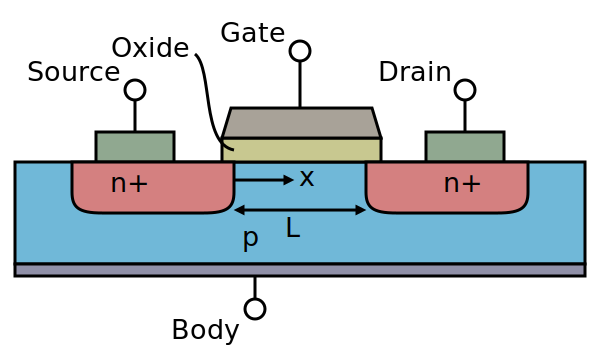
\includegraphics[width=0.50\textwidth]{./Rozdzial_3/obrazki/Lateral_mosfet}
	\caption{Przekrój ukazujący wewnętrzna budowę tranzystora typu MOSFET}
	\label{fig:MOSFET}
	\end{figure}

Jak widzimy na podłożu typu p zostały wytworzone obszary typu n, stanowiące źródło i dren. Zazwyczaj obszary te 
powstają na drodze implantacji jonów lub dyfuzji atomów domieszek do podłoża. Pomiędzy tymi obszarami w efekcie 
zjawiska polowego powstaje kanał. Kanał tworzy  się, gdy pomiędzy bramkę a podłoże zostanie przyłożone napięcie. 
Dla tranzystora typu n-kanałowego, napięcie musi być dodatnie. Po przyłożeniu dodatniego napięcia, elektrony 
z podłoża zaczynają gromadzić się pod bramką. W ten sposób jako nośniki mniejszościowe sprawiają, że obszar ten
staje się obszarem wyróżnionym pod względem zwiększenia jego przewodności. Dzięki temu przy przyłożonym napięciu 
pomiędzy drenem a źródłem zaczyna płynąć prąd. 

Taki tranzystor może znajdować się w 3 obszarach pracy. Wyłączony, brak wytworzonego kanału, duża oporność pomiędzy
drenem i źródłem. Obszar liniowej pracy kiedy to prąd drenu zależy w przybliżeniu liniowo od napięcia dren-źródło. 
Wreszcie obszar nasycenia, gdzie prąd źródło-dren słabo zależy od zmian napięcia pomiędzy nimi. Wszystkie te sytuacje
przedstawia rysunek \ref{fig:MOSFET_char}.


	\begin{figure}[ht]
	\centering
	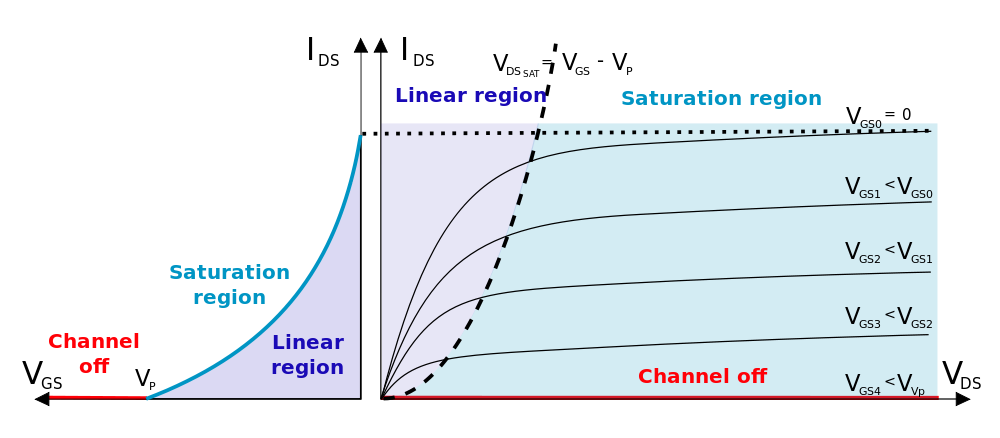
\includegraphics[width=0.90\textwidth]{./Rozdzial_3/obrazki/Charakterystyki_FET}
	\caption{Zależność prądu płynącego przez tranzystor}
	\label{fig:MOSFET_char}
	\end{figure}

Matematycznie można to opisać równaniem:

\begin{equation}
    \mathrm{ I_{DS}(V_G, V_{DS}) = \mu C_{ox} \frac{W}{L}[(V_G - V_T)V_{DS} - \frac{V_{DS}^2}{2}]}
	\label{equ:prad_drenu}
\end{equation}

Wyróżniamy dwa podstawowe typy charakterystyk elektrycznych tranzystorów FET. Pierwszym jest charakterystyka przejściowa,
którą otrzymuje się gdy prąd drenu otrzymuje się jako funkcję napięcia bramkowego, przy stałym napięciu źródło-dren. 
Drugim typem jest tak zwana charakterystyka wyjściowa będąca funkcją prądu drenu do napięcia dren-źródło, przy stałym 
napięciu bramkowym.

Mierząc te charakterystyki i porównując je ze wzorem \ref{equ:prad_drenu}, można wyznaczyć ruchliwość badanego tranzystora, $\mu$. 
Znając inne parametry występujące we wzorze, gdzie: L-długość kanału, W-szerokość kanału, 
$\mathrm {C_{ox}}$-powierzchniowa gęstość
 pojemności pomiędzy kanałem a bramką, $\mathrm{ V_G}$-napięcie bramkowe,
 $\mathrm{ V_{DS}}$-napięcie dren-źródło, $\mathrm{ V_T}$-tak zwane napięcie progowe.
Pomiary tych charakterystyk stały się podstawą do wyciągnięcia wniosków o właściwościach transportowych grafenu, użytego
w roli kanału.

Dzisiaj w świecie inżynierii elektronicznej istnieją dwie podstawowe grupy określające zastosowanie danego tranzystora. 
Zastosowania w układach logicznych lub w układach radiowych. W zasadzie można powiedzieć, że albo do zastosowań cyfrowych
albo do zastosowań analogowych. 

Relatywnie większą łatwość wprowadzania nowych technologicznie materiałów obserwuje się w segmencie analogowym. Wynika, to
głównie z tego względu, że wydajność urządzeń cyfrowych najbardziej zależy od najgorszych egzemplarzy tranzystorów 
zintegrowanych w układzie logicznym. Podczas, gdy w przypadku pojedynczo produkowanych tranzystorów do zastosowań analogowych,
te z nich, które za bardzo odbiegają parametrami od norm mogą zostać niedopuszczone do sprzedaży. Co odbywa się bez wpływu
dla reszty sprzedawanych egzemplarzy tranzystorów.

Jednak pomimo różnic, obie te gałęzie dążą do wspólnych celów. Zmniejszenia kosztów produkcji pojedynczego tranzystora.
Polepszenia jego właściwości. Głównie dla tranzystorów przeznaczonych do zastosowań cyfrowych działaniem mającym na celu
 zaspokojenie obu tych wymagań przez wiele lat było sukcesywne zmniejszanie pojedynczego tranzystora. Dzięki temu stawały
 się one szybsze. Zajmując mniej miejsca na podłożu oszczędzały drogi krzem.

Dzięki tym zabiegom złożoność układów cyfrowych mogła się podwajać co 18 miesięcy. Ta zależność jest nazywana ,,prawem
Moora". Jednocześnie takie układy stawały się tańsze.

Ze zmniejszaniem się pojedynczego tranzystora rosły wymagania co do procesu technologicznego, w którym je produkowano.
Dzisiejsze fabryki układów scalonych stały się niesłychanie kosztownymi przedsięwzięciami (kosztującymi miliardy dolarów).
Właśnie te linie produkcyjne są jednym z powodów całkowitego opanowania przez krzem technologii produkcji układów
 cyfrowych, ponieważ budowa nowej fabryki pochłonie więcej pieniędzy niż modernizacja obecnej. Należy pamiętać, że postępem
rządzi ekonomia.

To rozwiązanie zaczęło zawodzić, kiedy zaczęto dochodzić rozmiarami tranzystora do granic możliwości. Wtedy stało się jasne,
że niezbędne będzie opracowanie całkowicie nowej technologii wytwarzania lepszych tranzystorów.


Sytuacja w dziedzinie zastosowań analogowych, ze szczególnym wskazaniem zastosowań radiowych, wygląda z goła inaczej. 
Tutaj sama miniaturyzacja tranzystora nie jest najważniejsza, bo ważniejsze są jego właściwości, a same zintegrowane układy
analogowe są znacznie bardziej proste niż cyfrowe. Dodatkowo badania nad wieloma technologiami były i są wspierane przez
 agencje wojskowe. Dzięki temu produkty wysokiej jakości, ale będące drogie znajdują swoje zastosowania. Dzięki temu ten
 segment rynku jest znacznie bardziej otwarty na nowe technologie. Jako przykłady można wspomnieć tutaj np o tranzystorach
HEMT, opartych na materiałach III-IV; urządzeniach opartych na technologii arsenku galu GaAs, lub fosforku indu InP.

Podsumowując, z powodów tutaj przedstawionych wynika, że technologia grafenu ma większą szansę zaistnieć 
w wysokoczęstotliwościowych zastosowaniach analogowych. Dodatkowe argumenty potwierdzające tą tezę znajdują się 
w kolejnej części, mówiącej o czysto fizycznych aspektach stosowania grafenu do produkcji urządzeń elektronicznych.

	\section{Tranzystor FET z kanałem grafenowym}
		\subsection{Podstawy fizyczne działania}	
			Opis zasady działania, dla grafenu.
		\subsection{Najważniejsze właściwości}
			\paragraph{Ruchliwość}
			\paragraph{Przerwa energetyczna}
			\paragraph{Definicje najważniejszych parametrów}
		\subsection{Omówienie charakterystyk elektrycznych}


	\section{Proces produkcji tranzystorów z kanałem grafenowym}
		\subsection{Struktury tranzystorów}
		\subsection{Metoda produkcji tranzystorów}
			\paragraph{Opis metodologii}
			\paragraph{Zdjęcia optyczne}
